%The executive summary is a special chapter before the TOC
% See the other sections (e.g. Context) for more normal chapter headings
%%%%%%%%%%%%%%%%%%%%%%%%%%%%%%%%%%%%
\todo{Call it Front Matter in TOC, as it will include Glossary and auto-generated TOC, LOF.}
\chapterimage{ChapterImages/teaser} % Chapter heading image
\chapter[Front Matter]{Executive Summary} 
\label{cha:front}
%\addcontentsline{toc}{section}{Executive Summary}
%%%%%%%%%%%%%%%%%%%%%%%%%%%%%%%%%%%%
%Begin the actual executive summary text. If you create any subsections you
%probably want to use  \section*{Section name}  with an asterisk, so they are not numbered.
% Note: to get proper looking quotes use two left/right single quotes: ``. . . ''

%%%%%%Example of a remark that can optionally be printed:
% \begin{remark}\color{blue}
% \emph{(To hide these blue remarks, set} \verb'commentson' \emph{in AUDI\_FallDoc.tex)}

% Suggested length of this section: 2-2.5 pages including figure(s).
% \noindent This the most important section to edit carefully. It should stand alone. Assume it is the \emph{only} section that your
% corporate liaison's boss will read.
% \begin{itemize} %\tightlist   % a list with reduced white space
% \item Introduce the reader to what your project is about. 
% \item You can use your Fall Brochure as a starting point.
% \item Say something brief to introduce the design team (local + global).
% \item Motivate the current project direction (based on findings from users and experts,
% benchmarking, CEP or CFP, etc.).
% \item What you did is less important than \textbf{what you learned}.  What findings or insights do you have?
% \item Make sure your current ``Point of View'' comes across. The person who reads only the Executive
% Summary should still have an idea who your User is.
% \item Include images that capture the gist of your design problem and vision.
% If an image from your CFP, CEP is helpful, use it! Because this is a stand-alone section, it's fine
% to duplicate any images from this section elsewhere in the main document.
% \end{itemize}

% The remainder of this section is taken from 
% %\cite{Autodesk2008Fall}
% , a pretty good Fall document, done in Latex.
% \normalcolor
% \end{remark}
% %%%%End of remark


%%%%%%%%%%%%%%%%%%BEGIN EXAMPLE TEXT FOR THIS SECTION %%%%%%%%%%%%
\lettrine[lines=2]{W}{\ \ hat} are people most concerned with during their transition between home and being on their way? When leaving their home and upon arriving, people have a set list of things to keep in mind: ``Did I pack everything I will need for the day?'' is one crucial aspect that becomes most pressing before leaving, while ``How can I quickly disarm my alarm system and make sure I don't forget about it?'' becomes relevant upon return. Our set goal is to make this transition easier for Audi customers, to support them in what they already do, to remind them of things they forgot and to put them in control of what happens when.
% We therefore propose two different systems that both take a smart home and a smart car as given circumstances. We strongly believe that the coming 3 to 5 years will bring more interconnectedness, making available open connections to a variety of smart devices such as alarm systems, window and door sensors, as well as data around the car's status.

To make this possible, we propose a device we call AudiSeamless. It addresses two main concerns users have around their departure from and arrival to their home. 
\begin{enumerate}
    \item Upon \textbf{departure,} helps users remember about things they need to take care of before leaving.
    \item Upon \textbf{arrival,} helps users to disarm their alarm system in a secure and user-friendly way.
\end{enumerate}


\begin{figure}
  \centering
    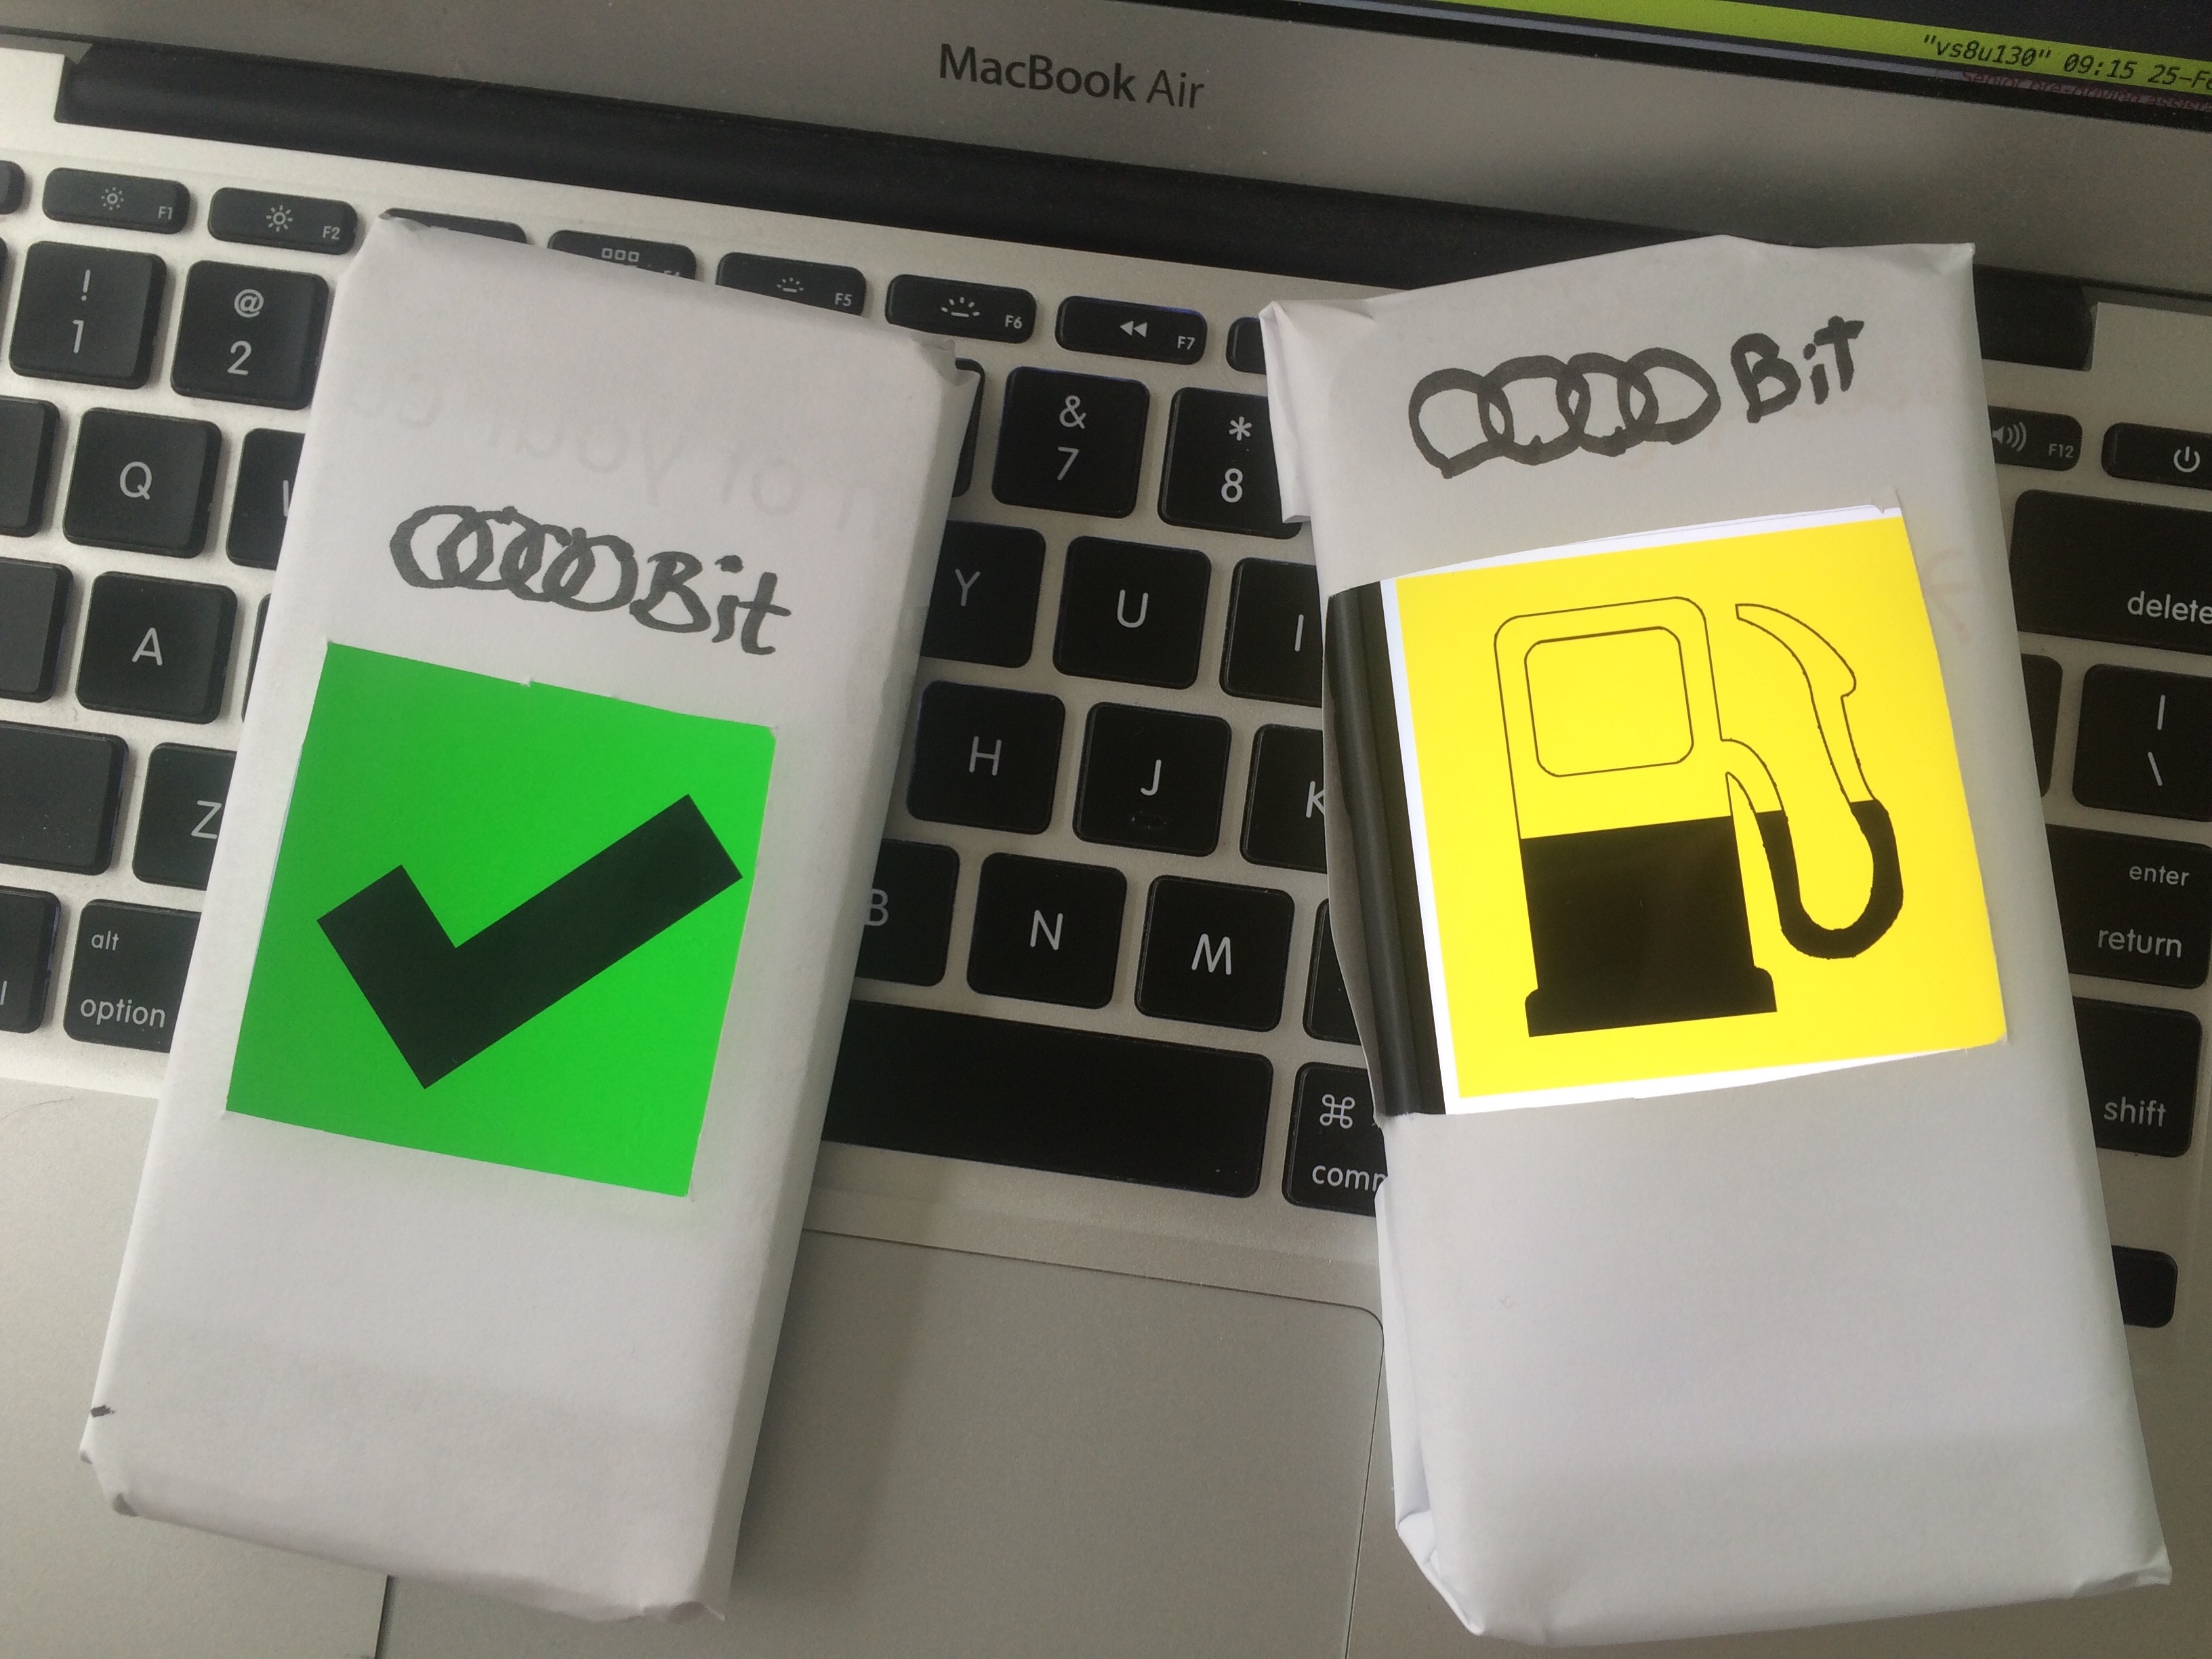
\includegraphics[width=1.0\textwidth]{Figures/AudiBits.JPG}
  \caption{Two \textbf{AudiBits}, the left one displaying an item that the user has packed, the right one displaying the amount of gas left in a user's car.}
  \label{fig:audi_bits_summary}
\end{figure}

\paragraph*{1. Departure} Our main functionality upon departure makes people less forgetful by collecting and making available information to its users about smart home and smart car utilities, as well as personal items, in a meaningful way. This functionality is the result of user interviews and testings, during which we heard that many of those users are forgetful about things like packing, putting their home in a state that enables them to leave, or about things related to their car, like its gas status or where it is parked. AudiSeamless enables display devices like smart phones to ``subscribe'' to utilities and personal items so they get fed with the current status of those. One possible application of this lies in our idea named \textbf{AudiBits}, small displays that show the status of singular items, for example the amount of gas left in a car or whether a user has packed his umbrella (see figure \ref{fig:audi_bits_summary}). Users can specify what AudiBits display, AudiBits in turn suggest useful actions that help users in their daily routine. If an AudiBit detects icy weather and that a user's car is parked outside, it suggests pre-heating the windows so the car owner won't lose time defrosting them. This semi-automation that gives clever suggestions but leaves the user in control is a major aspect of the system and, going forward, we want to further explore its usefulness and applications with users.

\paragraph*{2. Arrival} Upon arrival, AudiSeamless disarms a user's home security system easily by using the presence of a user's car key fob. When a user returns home, all she has to do is place her key fob in a bowl or near a sensor to deactivate the alarm, instead of entering a code, as is standard with current systems.
% {Jonathan} Not relevant for the high-level picture. Here, we only want to show our idea. If somebody is interested in details, they have to read the fine print aka the rest of the document
% Some systems do have wireless key fobs, but the long range signals could easily be intercepted by home invaders and used to deactivate the system.
Owners of home alarm systems produce a lot of false alarms since disarming the system has to be done quickly and can easily result in errors. As a result, many home security systems go unused due to the danger of false alarms, which cost money in public services as well as fines for the homeowner. Our aim with AudiSeamless is to reduce false alarms so that home owners will have reduced costs and lose the urge to disable their alarm system.

% {Jonathan} I think this is too detailed for the executive summary
Users expressed significant interest in having a reason to keep their keys in the same place every day, so that they know exactly where they are. At the moment, there is nothing that ties users' keys to a specific location, so they are often misplaced. Our system should be able to work for both the case if users take their keys out of their pockets when walking in their front door, as well as if they choose to keep them in a bag or purse, as is common with Audi smart key systems, which do not require being placed into a specific place within the car. Only the presence inside of the car is required. Similarly, such a presence inside the home could signal to the home security system that the owner is home. As key fobs are relatively secure and dedicated electronics that verify a user's identity, they offer a convenient and secure way to incorporate smart home functionality into the home through the owner's car, but without compromising integrity of their home lives.

One potential benefit of AudiSeamless is to signal the intent of the Audi owner to their car that they are about to leave. This allows the car to heat up (including electric batteries, which function much more efficiently when heated), connect to the internet to download preloaded directions, and prepare the car's climate if in hot or cold weather. As the user picks up their key fob, the system can send the intention of leaving to the car, and at the same time, a display can remind the user to bring certain belongings if they are not already packed.

These approaches demonstrate a departure from forcing integration with the smart home technology explored last quarter which, while interesting, did not address compelling latent user needs in the team's opinion. Our exploration of the design space this quarter stretches significantly more broadly than last quarter to search for more compelling user needs. However, we believe that we can enhance the experience of arriving and leaving home, specifically addressing the desires of Audi users to have systems that are simple, elegant, not pretentious or showy, and secure.

\begin{figure}[ht]
\label{Fig.AudiDefender}
\centering
	\includegraphics[keepaspectratio, width=5in]{Figures/Specifications/AudiDefender.JPG}
	\caption{The AudiSeamless arrival prototype tested the home security system deactivation with a key fob. The embedded touch screen displayed basic information, analogous to the AudiBits prototype, about the user's car and home.}
\end{figure}